\subsection{Introduction}\label{subsec:introduction_base_de_donnee}
Dans le cadre de mon application Clever Party Thrower, une base de données est utilisée pour gérer les différentes données générées par les utilisateurs et nécessaires au bon fonctionnement de l'application.
Dans cette section, je vais détailler les différents aspects de la base de données et comment ils ont été mis en œuvre dans le projet.

\subsection{Choix de la base de données}\label{subsec:choix-de-la-base-de-donnee}
Le choix du système de base de données est crucial car il détermine une grande partie du fonctionnement et des performances de l'application.
Comme déjà discuté dans l'analyse, j'ai choisi d'utiliser une base de données de type SQL et plus précisément PostgreSQL. L'utilisation de PostgreSQL me permet d'assurer la haute disponibilité de la base de données, si nécessaire, grâce à ses fonctionnalités de réplication des données.

Mais c'est surtout l'extensibilité de PostgreSQL qui était intéressante pour ce projet.
En effet, le système d'addons de PostgreSQL permet d'ajouter des fonctionnalités à la base de données assez simplement.
L'addon qui m'intéressait le plus dans mon cas est PostGIS car il permet de stocker et de manipuler des données de type point géographique.
Grâce à PostGIS, ma base de données est capable de calculer directement la distance entre deux points géographiques.

De plus, l'aspect open-source de PostgreSQL et sa réputation en font le candidat idéal pour mon projet.
De plus, les performances de PostgreSQL sont très bonnes, ce qui est essentiel pour assurer la fluidité de l'expérience utilisateur.

Enfin, la compatibilité de PostgreSQL avec de nombreux langages de programmation et ORMs,
dont TypeOrm que j'ai utilisé pour le développement de l'application, a également été un facteur déterminant dans mon choix.

\subsection{Structure de donnees}\label{subsec:structure-de-donnees}
voici la structure de la base de donnee.
\begin{figure}[h!]
    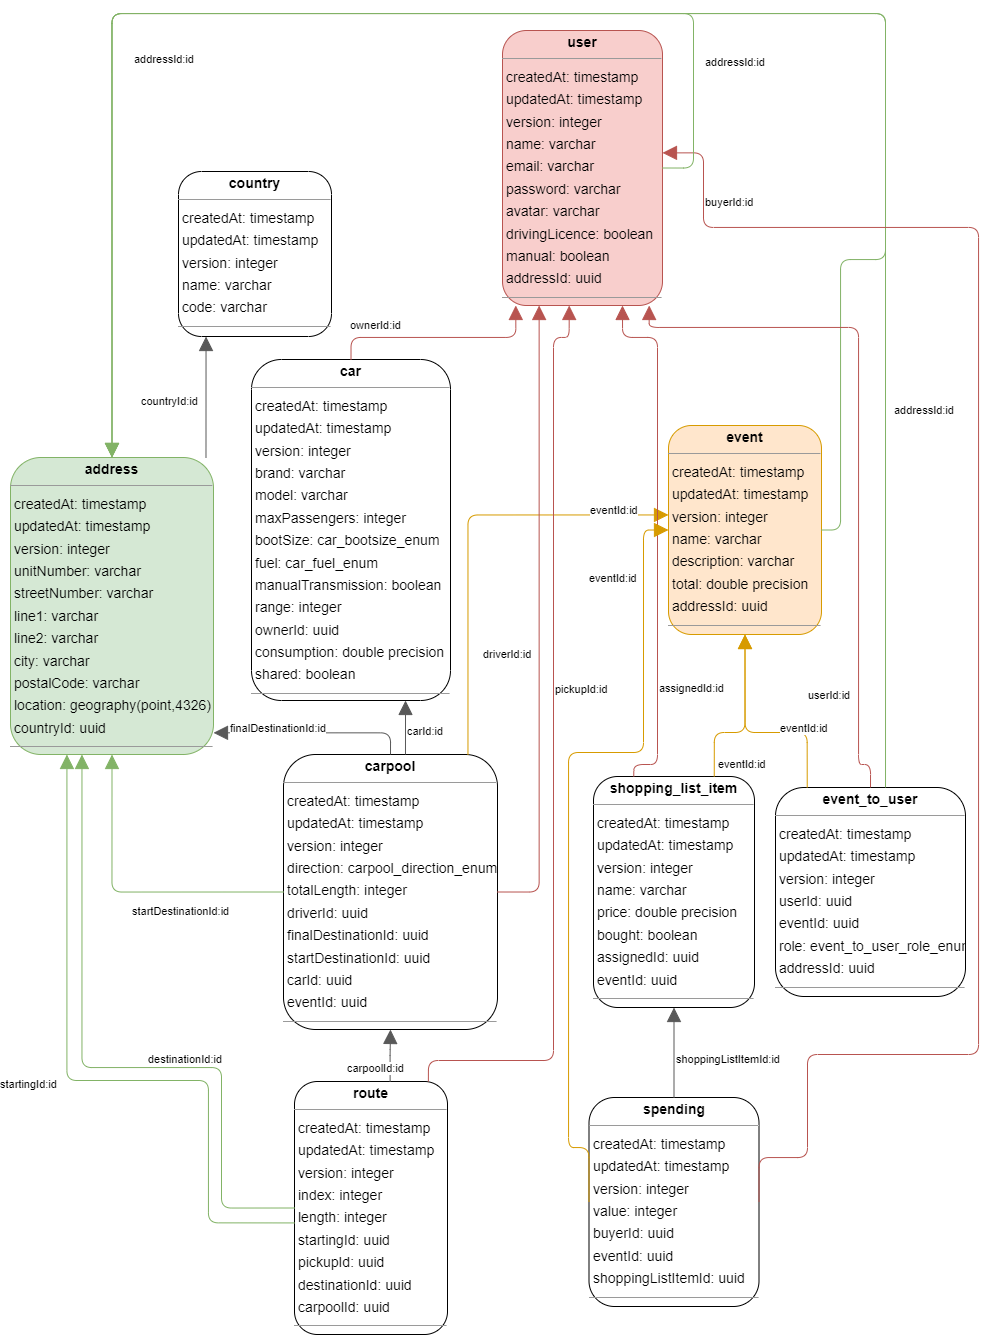
\includegraphics[width=\linewidth]{./images/dbShema}\caption{Architecture de la base de donnée}\label{fig:dbSchema2}
    \centering
\end{figure}
